%
% sudoku.tex
%
% (c) 2026 Nathanael Fässler, OST Ostschweizer Fachhochschule
%
% !TEX root = ../../buch.tex
% !TEX encoding = UTF-8
%

% Hilfsfunktion um Sudokus zu zeichnen
\newcounter{sudokuRow}
\newcounter{sudokuCol}

\newcommand\setrow[4]{
  \setcounter{sudokuCol}{1}
  \foreach \n in {#1, #2, #3, #4} {
    \edef\x{\value{sudokuCol} - 0.5}
    \edef\y{4.5 - \value{sudokuRow}}
    \node[anchor=center, font=\Huge] at (\x, \y) {\n};
    \stepcounter{sudokuCol}
  }
  \stepcounter{sudokuRow}
}

\section{Sudoku
\label{buchberger:section:sudoku}}
\kopfrechts{Sudoku}

\begin{figure}
\centering
\input{papers/buchberger/images/sudokuUnsolved.tex}
\caption{Ein ungelöstes Sudoku.
\label{buchberger:sudokuUnsolved}}
\end{figure}
Ein Sudoku ist ein bekanntes Ausfüllrätsel, bei dem in jedes leere Feld eine Ziffer eingetragen werden muss.
Das Sudoku gilt als gelöst wenn bestimmte Regeln erfüllt sind.

Das abgebildete 4x4 Sudoku\footnote{Ein 4x4 Sudoku wird auch Shidoku genannt.} ist eine kleinere Form des üblichen 9x9 Sudokus.
Die Regeln sind gleich, aber auf die kleinere Form angepasst.
Die Struktur und Regeln eines Sudokus lassen sich mathematisch mit Gleichungen einfach modellieren.
Deshalb bietet es sich an, die Anwendung des Buchberger-Algorithmus anhand eines Sudokus zu demonstrieren.

\subsection{Variablen des Sudokus
\label{buchberger:subsection:variablen-des-sudokus}}
\begin{figure}
\centering
\input{papers/buchberger/images/sudokuVariables.tex}
\caption{Sudoku mit Variablen für alle 16 Felder.
\label{buchberger:sudokuVariables}}
\end{figure}Zunächst müssen die Variablen des Gleichungssystem definiert werden.
Für jedes Feld im Sudoku gibt es eine Variable $x_{ij}$ mit den Indizes $i, j \in \{1, 2, 3, 4\}$, wobei $i$ die Spalte und $j$ die Zeile identifiziert.
In~\ref{buchberger:sudokuVariables} ist jede Variable in ihrem Feld eingezeichnet.
Der Wert einer Variablen steht für die Ziffer die an ihrem Feld eingetragen werden soll.

\subsection{Gleichungen des Sudokus
\label{buchberger:subsection:gleichungen-des-sudokus}}
\subsubsection{Regel 1: Jedes Feld muss entweder 1, 2, 3 oder 4 sein.}
Um diese Regel mit Gleichungen darzustellen wird zunächst das Problem in kleinere Teilprobleme zerlegt.
Wenn man nur $x_{11}$ isoliert betrachtet kann man festhalten:
Das Feld $x_{11}$ muss 1, 2, 3 oder 4 sein.

Es wird also eine Gleichung benötigt, welche die Lösungsmenge
\[
L = \{1, 2, 3, 4\}
\]
hat.
Dies wird durch die Gleichung
\begin{equation}
  (x_{11} - 1)\,(x_{11} - 2)\,(x_{11} - 3)\,(x_{11} - 4) = 0
  \label{buchberger:sudoku-gleichung-1}
\end{equation}
erzwungen. Wenn einer der 4 Faktoren 0 ergibt, wird die ganze Gleichung erfüllt.

Wenn man es noch für die restlichen 15 Variablen anwendet ergeben sich die Gleichungen
\begin{equation}
  (x_{12} - 1)\,(x_{12} - 2)\,(x_{12} - 3)\,(x_{12} - 4) = 0
  \label{buchberger:sudoku-gleichung-2}
\end{equation}
\begin{equation}
  (x_{13} - 1)\,(x_{13} - 2)\,(x_{13} - 3)\,(x_{13} - 4) = 0
  \label{buchberger:sudoku-gleichung-3}
\end{equation}
\begin{equation}
  (x_{14} - 1)\,(x_{14} - 2)\,(x_{14} - 3)\,(x_{14} - 4) = 0
  \label{buchberger:sudoku-gleichung-4}
\end{equation}
\begin{equation}
  (x_{21} - 1)\,(x_{21} - 2)\,(x_{21} - 3)\,(x_{21} - 4) = 0
  \label{buchberger:sudoku-gleichung-5}
\end{equation}
\begin{equation}
  (x_{22} - 1)\,(x_{22} - 2)\,(x_{22} - 3)\,(x_{22} - 4) = 0
  \label{buchberger:sudoku-gleichung-6}
\end{equation}
\begin{equation}
  (x_{23} - 1)\,(x_{23} - 2)\,(x_{23} - 3)\,(x_{23} - 4) = 0
  \label{buchberger:sudoku-gleichung-7}
\end{equation}
\begin{equation}
  (x_{24} - 1)\,(x_{24} - 2)\,(x_{24} - 3)\,(x_{24} - 4) = 0
  \label{buchberger:sudoku-gleichung-8}
\end{equation}
\begin{equation}
  (x_{31} - 1)\,(x_{31} - 2)\,(x_{31} - 3)\,(x_{31} - 4) = 0
  \label{buchberger:sudoku-gleichung-9}
\end{equation}
\begin{equation}
  (x_{32} - 1)\,(x_{32} - 2)\,(x_{32} - 3)\,(x_{32} - 4) = 0
  \label{buchberger:sudoku-gleichung-10}
\end{equation}
\begin{equation}
  (x_{33} - 1)\,(x_{33} - 2)\,(x_{33} - 3)\,(x_{33} - 4) = 0
  \label{buchberger:sudoku-gleichung-11}
\end{equation}
\begin{equation}
  (x_{34} - 1)\,(x_{34} - 2)\,(x_{34} - 3)\,(x_{34} - 4) = 0
  \label{buchberger:sudoku-gleichung-12}
\end{equation}
\begin{equation}
  (x_{41} - 1)\,(x_{41} - 2)\,(x_{41} - 3)\,(x_{41} - 4) = 0
  \label{buchberger:sudoku-gleichung-13}
\end{equation}
\begin{equation}
  (x_{42} - 1)\,(x_{42} - 2)\,(x_{42} - 3)\,(x_{42} - 4) = 0
  \label{buchberger:sudoku-gleichung-14}
\end{equation}
\begin{equation}
  (x_{43} - 1)\,(x_{43} - 2)\,(x_{43} - 3)\,(x_{43} - 4) = 0
  \label{buchberger:sudoku-gleichung-15}
\end{equation}
\begin{equation}
  (x_{44} - 1)\,(x_{44} - 2)\,(x_{44} - 3)\,(x_{44} - 4) = 0
  \label{buchberger:sudoku-gleichung-16}
\end{equation}
.

\subsubsection{Regel 2: Die vorgegebenen Felder dürfen nicht verändert werden.}
Die Gleichungen
\begin{equation}
  x_{13} = 2
  \label{buchberger:sudoku-gleichung-17}
\end{equation}
\begin{equation}
  x_{31} = 3
  \label{buchberger:sudoku-gleichung-18}
\end{equation}
\begin{equation}
  x_{34} = 1
  \label{buchberger:sudoku-gleichung-19}
\end{equation}
\begin{equation}
  x_{42} = 4
  \label{buchberger:sudoku-gleichung-20}
\end{equation}
sind trivial.

Dadurch wurden die Gleichungen 
\eqref{buchberger:sudoku-gleichung-3}, 
\eqref{buchberger:sudoku-gleichung-9},
\eqref{buchberger:sudoku-gleichung-12} und 
\eqref{buchberger:sudoku-gleichung-14} 
redundant.
Dies ist jedoch kein Problem, da redundante Gleichungen keine Widersprüche erzeugen und am Schluss ohnehin entfernt werden.

\subsubsection{Regel 3: In jeder Zeile muss jede Zahl genau einmal stehen.}
Auch hier wird sich Abhilfe geschaffen, indem nur ein Teilproblem auf einmal gelöst wird:
Zum Beispiel muss in der obersten Zeile die Zahl 1 mindestens einmal vorkommen.
Die Gleichung
\begin{equation}
  (x_{11} - 1)\,(x_{12} - 1)\,(x_{13} - 1)\,(x_{14} - 1) = 0
  \label{buchberger:sudoku-gleichung-21}
\end{equation}
bewirkt dies.

Die Gleichungen
\begin{equation}
  (x_{11} - 2)\,(x_{12} - 2)\,(x_{13} - 2)\,(x_{14} - 2) = 0
  \label{buchberger:sudoku-gleichung-22}
\end{equation}
\begin{equation}
  (x_{11} - 3)\,(x_{12} - 3)\,(x_{13} - 3)\,(x_{14} - 3) = 0
  \label{buchberger:sudoku-gleichung-23}
\end{equation}
\begin{equation}
  (x_{11} - 4)\,(x_{12} - 4)\,(x_{13} - 4)\,(x_{14} - 4) = 0
  \label{buchberger:sudoku-gleichung-24}
\end{equation}
stellen sicher, dass auch die Zahlen 2, 3 und 4 in der obersten Zeile vorkommen.

Der aufmerksame Leser hat vielleicht gemerkt, dass die Teilregel nur verlangt, dass eine Zahl mindestens einmal vorkommt und nicht, dass eine Zahl genau einmal vorkommt.
Somit ist z.B. die Gleichung \eqref{buchberger:sudoku-gleichung-21} auch erfüllt, wenn die ganze obere Zeile nur aus Einsen besteht.
Jedoch erfüllen die 4 Gleichungen der Zeile zusammen trotzdem die Regel.
Der einzige Weg alle 4 Gleichungen gleichzeitig zu erfüllen besteht darin, dass jede Zahl genau einmal vorkommt.
Wenn z.B. zwei Einsen in der obersten Zeile stünden, würde zwangsläufig eine andere Gleichung verletzt werden, da z.B. die Vier fehlt.
Der Buchberger-Algorithmus wird gezwungen eine Lösung zu finden wo jede Zahl genau einmal vorkommt, sonst kann er nicht alle Gleichungen gleichzeitig erfüllen.

Die restlichen Gleichungen folgen dem gleichen System:
\begin{equation}
  (x_{21} - 1)\,(x_{22} - 1)\,(x_{23} - 1)\,(x_{24} - 1) = 0
  \label{buchberger:sudoku-gleichung-25}
\end{equation}
\begin{equation}
  (x_{21} - 2)\,(x_{22} - 2)\,(x_{23} - 2)\,(x_{24} - 2) = 0
  \label{buchberger:sudoku-gleichung-26}
\end{equation}
\begin{equation}
  (x_{21} - 3)\,(x_{22} - 3)\,(x_{23} - 3)\,(x_{24} - 3) = 0
  \label{buchberger:sudoku-gleichung-27}
\end{equation}
\begin{equation}
  (x_{21} - 4)\,(x_{22} - 4)\,(x_{23} - 4)\,(x_{24} - 4) = 0
  \label{buchberger:sudoku-gleichung-28}
\end{equation}
\begin{equation}
  (x_{31} - 1)\,(x_{32} - 1)\,(x_{33} - 1)\,(x_{34} - 1) = 0
  \label{buchberger:sudoku-gleichung-29}
\end{equation}
\begin{equation}
  (x_{31} - 2)\,(x_{32} - 2)\,(x_{33} - 2)\,(x_{34} - 2) = 0
  \label{buchberger:sudoku-gleichung-30}
\end{equation}
\begin{equation}
  (x_{31} - 3)\,(x_{32} - 3)\,(x_{33} - 3)\,(x_{34} - 3) = 0
  \label{buchberger:sudoku-gleichung-31}
\end{equation}
\begin{equation}
  (x_{31} - 4)\,(x_{32} - 4)\,(x_{33} - 4)\,(x_{34} - 4) = 0
  \label{buchberger:sudoku-gleichung-32}
\end{equation}
\begin{equation}
  (x_{41} - 1)\,(x_{42} - 1)\,(x_{43} - 1)\,(x_{44} - 1) = 0
  \label{buchberger:sudoku-gleichung-33}
\end{equation}
\begin{equation}
  (x_{41} - 2)\,(x_{42} - 2)\,(x_{43} - 2)\,(x_{44} - 2) = 0
  \label{buchberger:sudoku-gleichung-34}
\end{equation}
\begin{equation}
  (x_{41} - 3)\,(x_{42} - 3)\,(x_{43} - 3)\,(x_{44} - 3) = 0
  \label{buchberger:sudoku-gleichung-35}
\end{equation}
\begin{equation}
  (x_{41} - 4)\,(x_{42} - 4)\,(x_{43} - 4)\,(x_{44} - 4) = 0
  \label{buchberger:sudoku-gleichung-36}
\end{equation}


\subsubsection{Regel 4: In jeder Spalte muss jede Zahl genau einmal stehen.}
Diese Regel funktioniert analog zu Regel 3.
\begin{equation}
  (x_{11} - 1)\,(x_{21} - 1)\,(x_{31} - 1)\,(x_{41} - 1) = 0
  \label{buchberger:sudoku-gleichung-37}
\end{equation}
\begin{equation}
  (x_{11} - 2)\,(x_{21} - 2)\,(x_{31} - 2)\,(x_{41} - 2) = 0
  \label{buchberger:sudoku-gleichung-38}
\end{equation}
\begin{equation}
  (x_{11} - 3)\,(x_{21} - 3)\,(x_{31} - 3)\,(x_{41} - 3) = 0
  \label{buchberger:sudoku-gleichung-39}
\end{equation}
\begin{equation}
  (x_{11} - 4)\,(x_{21} - 4)\,(x_{31} - 4)\,(x_{41} - 4) = 0
  \label{buchberger:sudoku-gleichung-40}
\end{equation}
\begin{equation}
  (x_{12} - 1)\,(x_{22} - 1)\,(x_{32} - 1)\,(x_{42} - 1) = 0
  \label{buchberger:sudoku-gleichung-41}
\end{equation}
\begin{equation}
  (x_{12} - 2)\,(x_{22} - 2)\,(x_{32} - 2)\,(x_{42} - 2) = 0
  \label{buchberger:sudoku-gleichung-42}
\end{equation}
\begin{equation}
  (x_{12} - 3)\,(x_{22} - 3)\,(x_{32} - 3)\,(x_{42} - 3) = 0
  \label{buchberger:sudoku-gleichung-43}
\end{equation}
\begin{equation}
  (x_{12} - 4)\,(x_{22} - 4)\,(x_{32} - 4)\,(x_{42} - 4) = 0
  \label{buchberger:sudoku-gleichung-44}
\end{equation}
\begin{equation}
  (x_{13} - 1)\,(x_{23} - 1)\,(x_{33} - 1)\,(x_{43} - 1) = 0
  \label{buchberger:sudoku-gleichung-45}
\end{equation}
\begin{equation}
  (x_{13} - 2)\,(x_{23} - 2)\,(x_{33} - 2)\,(x_{43} - 2) = 0
  \label{buchberger:sudoku-gleichung-46}
\end{equation}
\begin{equation}
  (x_{13} - 3)\,(x_{23} - 3)\,(x_{33} - 3)\,(x_{43} - 3) = 0
  \label{buchberger:sudoku-gleichung-47}
\end{equation}
\begin{equation}
  (x_{13} - 4)\,(x_{23} - 4)\,(x_{33} - 4)\,(x_{43} - 4) = 0
  \label{buchberger:sudoku-gleichung-48}
\end{equation}
\begin{equation}
  (x_{14} - 1)\,(x_{24} - 1)\,(x_{34} - 1)\,(x_{44} - 1) = 0
  \label{buchberger:sudoku-gleichung-49}
\end{equation}
\begin{equation}
  (x_{14} - 2)\,(x_{24} - 2)\,(x_{34} - 2)\,(x_{44} - 2) = 0
  \label{buchberger:sudoku-gleichung-50}
\end{equation}
\begin{equation}
  (x_{14} - 3)\,(x_{24} - 3)\,(x_{34} - 3)\,(x_{44} - 3) = 0
  \label{buchberger:sudoku-gleichung-51}
\end{equation}
\begin{equation}
  (x_{14} - 4)\,(x_{24} - 4)\,(x_{34} - 4)\,(x_{44} - 4) = 0
  \label{buchberger:sudoku-gleichung-52}
\end{equation}



\subsubsection{Regel 5: In jedem 2x2 Block muss jede Zahl genau einmal stehen.}
Diese Regel funktioniert auch wie die Regeln 3 und 4, aber anstatt Zeilen oder Spalten wird in jeder Gleichung einer der 2x2 Blöcke isoliert betrachtet.
\begin{equation}
  (x_{11} - 1)\,(x_{12} - 1)\,(x_{21} - 1)\,(x_{22} - 1) = 0
  \label{buchberger:sudoku-gleichung-53}
\end{equation}
\begin{equation}
  (x_{11} - 2)\,(x_{12} - 2)\,(x_{21} - 2)\,(x_{22} - 2) = 0
  \label{buchberger:sudoku-gleichung-54}
\end{equation}
\begin{equation}
  (x_{11} - 3)\,(x_{12} - 3)\,(x_{21} - 3)\,(x_{22} - 3) = 0
  \label{buchberger:sudoku-gleichung-55}
\end{equation}
\begin{equation}
  (x_{11} - 4)\,(x_{12} - 4)\,(x_{21} - 4)\,(x_{22} - 4) = 0
  \label{buchberger:sudoku-gleichung-56}
\end{equation}
\begin{equation}
  (x_{13} - 1)\,(x_{14} - 1)\,(x_{23} - 1)\,(x_{24} - 1) = 0
  \label{buchberger:sudoku-gleichung-57}
\end{equation}
\begin{equation}
  (x_{13} - 2)\,(x_{14} - 2)\,(x_{23} - 2)\,(x_{24} - 2) = 0
  \label{buchberger:sudoku-gleichung-58}
\end{equation}
\begin{equation}
  (x_{13} - 3)\,(x_{14} - 3)\,(x_{23} - 3)\,(x_{24} - 3) = 0
  \label{buchberger:sudoku-gleichung-59}
\end{equation}
\begin{equation}
  (x_{13} - 4)\,(x_{14} - 4)\,(x_{23} - 4)\,(x_{24} - 4) = 0
  \label{buchberger:sudoku-gleichung-60}
\end{equation}
\begin{equation}
  (x_{31} - 1)\,(x_{32} - 1)\,(x_{41} - 1)\,(x_{42} - 1) = 0
  \label{buchberger:sudoku-gleichung-61}
\end{equation}
\begin{equation}
  (x_{31} - 2)\,(x_{32} - 2)\,(x_{41} - 2)\,(x_{42} - 2) = 0
  \label{buchberger:sudoku-gleichung-62}
\end{equation}
\begin{equation}
  (x_{31} - 3)\,(x_{32} - 3)\,(x_{41} - 3)\,(x_{42} - 3) = 0
  \label{buchberger:sudoku-gleichung-63}
\end{equation}
\begin{equation}
  (x_{31} - 4)\,(x_{32} - 4)\,(x_{41} - 4)\,(x_{42} - 4) = 0
  \label{buchberger:sudoku-gleichung-64}
\end{equation}
\begin{equation}
  (x_{33} - 1)\,(x_{34} - 1)\,(x_{43} - 1)\,(x_{44} - 1) = 0
  \label{buchberger:sudoku-gleichung-65}
\end{equation}
\begin{equation}
  (x_{33} - 2)\,(x_{34} - 2)\,(x_{43} - 2)\,(x_{44} - 2) = 0
  \label{buchberger:sudoku-gleichung-66}
\end{equation}
\begin{equation}
  (x_{33} - 3)\,(x_{34} - 3)\,(x_{43} - 3)\,(x_{44} - 3) = 0
  \label{buchberger:sudoku-gleichung-67}
\end{equation}
\begin{equation}
  (x_{33} - 4)\,(x_{34} - 4)\,(x_{43} - 4)\,(x_{44} - 4) = 0
  \label{buchberger:sudoku-gleichung-68}
\end{equation}

\subsection{Sudoku lösen
\label{buchberger:subsection:sudoku-loesen}}
\begin{figure}
  \centering
  % (c) 2026 Nathanael Fässler, OST Ostschweizer Fachhochschule

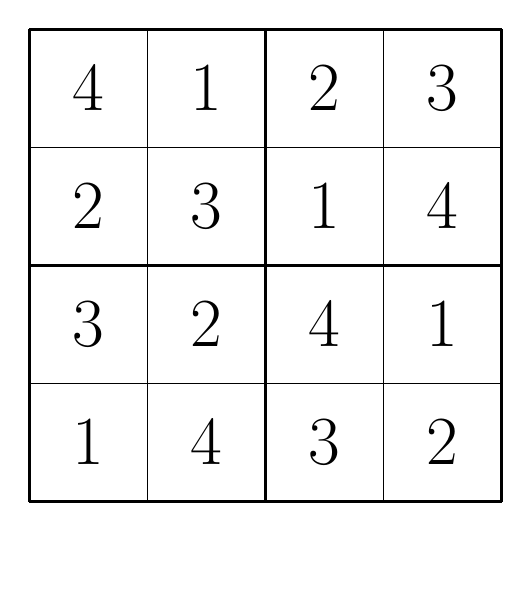
\begin{tikzpicture}[scale=1.5]
  \begin{scope}
  \draw (0,0) grid(4,4);
  \draw[very thick, scale=2] (0,0) grid (2, 2);

  \setcounter{sudokuRow}{1}
    \setrow {4}{1}  {2}{3}
    \setrow {2}{3}  {1}{4}

    \setrow {3}{2}  {4}{1}
    \setrow {1}{4}  {3}{2}
    \node[anchor=center] at (2, -0.5) {};
  \end{scope}

\end{tikzpicture}

  \caption{Das vom Buchberger-Algorithmus gelöste Sudoku.
  \label{buchberger:sudokuSolved}}
\end{figure}
Der Autor dieses Papers hat das Gleichungssystem mithilfe von \emph{Maxima}\footnote{Maxima ist ein Open-Source Computeralgebrasystem(CAS)} gelöst.
Dafür wurde die Funktion poly\_reduced\_grobner() mit allen 68 Gleichungen ausgeführt.
Es wurde eine lexikographische Ordnung verwendet.
Die Funktion führt den Buchberger Algorithmus aus und räumt auch direkt die redundanten Polynome auf.
Der Output der Funktion ist die Gröbner-Basis
\[
G =
\{
  x_{13} - 2,
  x_{31} - 3,
  x_{34} - 1,
  x_{42} - 4,
  x_{44} - 2,
  x_{43} - 3,
  4 - x_{24},
  1 - x_{23},
  x_{12} - 1,
  x_{11} - 4,
  2 - x_{32},
  x_{41} - 1,
  3 - x_{14},
  2 - x_{21},
  4 - x_{33},
  3 - x_{22}
\}
\]
, welche sich zum Gleichungssystem
\begin{equation}
  \begin{cases}
    x_{11} - 4 = 0 \\
    x_{12} - 1 = 0 \\
    x_{13} - 2 = 0 \\
    x_{14} - 3 = 0 \\
    x_{21} - 2 = 0 \\
    x_{22} - 3 = 0 \\
    x_{23} - 1 = 0 \\
    x_{24} - 4 = 0 \\
    x_{31} - 3 = 0 \\
    x_{32} - 2 = 0 \\
    x_{33} - 4 = 0 \\
    x_{34} - 1 = 0 \\
    x_{41} - 1 = 0 \\
    x_{42} - 4 = 0 \\
    x_{43} - 3 = 0 \\
    x_{44} - 2 = 0
  \end{cases}
  \label{buchberger:sudoku-end-loesung}
\end{equation}
umformen lässt.
Daraus lassen sich die Lösungen direkt ablesen und in das Sudoku~\ref{buchberger:sudokuSolved} eintragen.

Damit ist die Demonstration abgeschlossen.
Es ist erstaunlich, dass man ein Sudoku durch ein Gleichungssystem beschreiben und mit dem Buchberger-Algorithmus lösen kann.